pdfoutput=1
\pdfoutput=1
% !TEX program = xelatex
\documentclass[12pt,a4paper]{article}

% ================================================================
% Packages
% ================================================================
\usepackage{amsmath,amssymb,amsthm}
\usepackage{mathtools}
\usepackage{bm}
\usepackage{graphicx}
\usepackage{hyperref}
\usepackage{geometry}
\usepackage{enumitem}
\usepackage{booktabs}
\usepackage{tikz}
\usepackage{xcolor}
\usepackage{cleveref}
\usepackage{bbm}
\usepackage{float}
\usepackage{setspace}
\usepackage{longtable}
\usepackage{makecell}
\usepackage{multirow}
\usepackage{listings}

\geometry{margin=2.5cm}
\onehalfspacing

% ================================================================
% Hyperref setup
% ================================================================
\hypersetup{
    colorlinks=true,
    citecolor=blue,
    urlcolor=blue,
    pdftitle={Spring},
    pdfauthor={SCX},
    pdfsubject={SCX Spring Multimodal Unified Framework},
}

% ================================================================
% Theorem environments
% ================================================================
\newtheorem{theorem}{Theorem}[section]
\newtheorem{lemma}[theorem]{Lemma}
\newtheorem{proposition}[theorem]{Proposition}
\newtheorem{corollary}[theorem]{Corollary}
\newtheorem{definition}[theorem]{Definition}
\newtheorem{conjecture}[theorem]{Conjecture}
\newtheorem{criterion}[theorem]{Criterion}

\theoremstyle{remark}
\newtheorem{remark}[theorem]{Remark}
\newtheorem{example}[theorem]{Example}
\newtheorem{protocol}[theorem]{Protocol}

% ================================================================
% Custom commands — Mathematics
% ================================================================
\newcommand{\R}{\mathbb{R}}
\newcommand{\C}{\mathbb{C}}
\newcommand{\Q}{\mathbb{Q}}
\newcommand{\Z}{\mathbb{Z}}
\newcommand{\F}{\mathbb{F}}
\newcommand{\N}{\mathbb{N}}
\newcommand{\E}{\mathbb{E}}
\newcommand{\Pbb}{\mathbb{P}}
\newcommand{\Var}{\mathrm{Var}}
\newcommand{\Cov}{\mathrm{Cov}}
\newcommand{\indep}{\perp\!\!\!\perp}
\newcommand{\loss}{\mathcal{L}}
\newcommand{\D}{\mathcal{D}}
\newcommand{\T}{\mathcal{T}}
\newcommand{\A}{\mathcal{A}}
\newcommand{\M}{\mathcal{M}}
\newcommand{\Fset}{\mathcal{F}}
\newcommand{\X}{\mathcal{X}}
\newcommand{\I}{\mathcal{I}}
\newcommand{\Ocal}{\mathcal{O}}

% ================================================================
% Custom commands — SCX Framework
% ================================================================
\newcommand{\SCX}{\textsc{SCX}}
\newcommand{\Spring}{\textsc{Spring}}
\newcommand{\Yajie}{\textsc{Yajie}}
\newcommand{\Cercis}{\textsc{Cercis}}
\newcommand{\Situs}{\textsc{Situs}}

\newcommand{\Mauto}{\ensuremath{M_t^{\text{auto}}}}
\newcommand{\Lyap}{\ensuremath{\Psi}}
\newcommand{\Dhash}{\ensuremath{\mathcal{H}(\D)}}
\newcommand{\ModalitySet}{\ensuremath{\mathbb{M}}}

\DeclareMathOperator{\sgn}{sgn}
\DeclareMathOperator{\diag}{diag}
\DeclareMathOperator{\spec}{spec}
\DeclareMathOperator{\rank}{rank}
\DeclareMathOperator{\Tr}{Tr}
\DeclareMathOperator{\argmax}{arg\,max}
\DeclareMathOperator{\argmin}{arg\,min}
\DeclareMathOperator{\Auditable}{Auditable}
\DeclareMathOperator{\Lip}{Lip}
\DeclareMathOperator{\Enc}{Enc}
\DeclareMathOperator{\Dec}{Dec}
\DeclareMathOperator{\Physics}{Physics}
\DeclareMathOperator{\Compute}{Compute}

% ================================================================
% Proof-status markers
% ================================================================
\newcommand{\rigorous}{\textnormal{\textbf{[]}}}
\newcommand{\heuristic}{\textnormal{\textbf{[]}}}
\newcommand{\openproblem}{\textnormal{\textbf{[]}}}
\newcommand{\honeststrike}{\textnormal{\textbf{[]}}}

% Honest critique marker
\newcommand{\honestcrit}[1]{%
    \textcolor{red}{\textbf{#1}}%
}

% ================================================================
% Title
% ================================================================
\title{\textbf{Spring\\[4pt]
}\\[8pt]
\large The Spring Multimodal Unified Framework:\\
A Training-Is-Audit Architecture for\\
Omni-Modal Large Models}
\author{SCX}
\date{202671}

\begin{document}

\maketitle

\begin{center}
\footnotesize
\textbf{} v1.0 \quad | \quad
\textbf{}  \quad | \quad
\textbf{} SCX — Spring
\end{center}

% ================================================================
% Abstract
% ================================================================
\begin{abstract}
\Spring{}——
\Spring{}

(1) ——DFT
——
(2) \Spring{}——
$M_t$(3) RAG\Spring{}
(4) \Yajie{}$M_t$
(5) \Cercis{}

\Spring{}\textbf{}
“”\Spring{}→\Spring{}→
\Yajie{}→\Cercis{}——
GPTClaudeGemini$M=1$UNDECLARED
\Spring{}born audited——

\textbf{} SpringYajieCercis

\end{abstract}

\tableofcontents
\newpage

% ================================================================
% 1. Introduction
% ================================================================
\section{}

\subsection{}

Large Language Models, LLMsGPT-2GPT-4ClaudeGemini
“”
\textbf{}




\begin{enumerate}[label=(\arabic*),itemsep=4pt]
    \item \textbf{} 
    
    
    
    \item \textbf{} GPT-4“”
    
    
    
    \item \textbf{} 
    “”——
    
\end{enumerate}

——
\textbf{}
——

\subsection{SCX}

\SCX{}~\\cite{scx_ml_audit,scx_hamiltonian,yajie_protocol}
$M=1$

\begin{enumerate}[label=\textbf{ \arabic*},leftmargin=*,itemsep=4pt]
    \item \textbf{SCX2}
    $M=1$——“”“”
    “”$M=1$
    
    \item \textbf{SCX1}
    $M>1$——
    $M$$M$
    
    \item \textbf{-SCX3}
    ——
    
\end{enumerate}

\textbf{}

\Spring{}

\subsection{Spring}

\Spring{}SCX——~\\cite{scx_spring_trainer}
Spring\Yajie{}$M_t$
“”

\Spring{}
\textbf{\Spring{}}——GPT
“”

\begin{itemize}[nosep]
    \item \textbf{} DFT
    \item \textbf{} 
    \item \textbf{} 
    \item \textbf{} 
\end{itemize}

\textbf{\Spring{}
“→→→→”}



\begin{definition}[Spring — ]\label{def:spring_framework}
\Spring{}
\begin{equation}\label{eq:spring_pipeline}
    \boxed{
    \text{Input} \xrightarrow{\Enc} \text{Physics} \xrightarrow{\Spring} \text{Reasoning} \xrightarrow{\Yajie} \text{Audit} \xrightarrow{\Cercis} \text{Output}
    }
\end{equation}

\Spring{}————
\textbf{}
\end{definition}

\subsection{}



\begin{itemize}[nosep]
    \item \textbf{Modality} ——DFT
    $\ModalitySet = \{m_1, m_2, \ldots, m_K\}$
    \item \textbf{Physics Layer} \Spring{}——
    \Spring{}DFT
    \item \textbf{Reasoning Layer} ——
    RAG
    \item \textbf{Audit Layer} \Yajie{}$M_t$\Cercis{}
    \item \textbf{Large Model} ——
    
\end{itemize}

\subsection{}

\begin{enumerate}[label=(\arabic*),itemsep=3pt]
    \item 2\Spring{}——
    \item 3——
    \item 4——\Spring{}
    \item 5——LLMRAG
    \item 6——\Yajie{}$M_t$
    \item 7——DFT
    \item 8——\Cercis{}
    \item 9——GPT/Claude/Gemini$M=1$UNDECLARED
    \item 10——
    \item 11
\end{enumerate}

\newpage

% ================================================================
% 2. Spring Unified Architecture
% ================================================================
\section{Spring}

\subsection{}

\Spring{}
\ref{fig:spring_architecture}

\begin{figure}[H]
\centering
\begin{tikzpicture}[node distance=2.0cm, auto,
    block/.style={rectangle, draw, minimum width=3.5cm, minimum height=0.9cm, align=center, rounded corners=4pt},
    arrow/.style={->, thick}]

    % Layer 1: Input
    \node[block, fill=blue!8] (input) { (Input Layer) \\
        \footnotesize  $\Enc_\theta$};
    
    % Layer 2: Physics
    \node[block, fill=green!8, below=of input] (physics) { (Physics Layer) \\
        \footnotesize \Spring{}  / DFT / MD};
    
    % Layer 3: Reasoning
    \node[block, fill=yellow!12, below=of physics] (reasoning) { (Reasoning Layer) \\
        \footnotesize LLM + RAG over \Spring{} outputs};
    
    % Layer 4: Audit
    \node[block, fill=orange!10, below=of reasoning] (audit) { (Audit Layer) \\
        \footnotesize \Yajie{}  / $M_t$  / };
    
    % Layer 5: Output
    \node[block, fill=red!8, below=of audit] (output) { (Output Layer) \\
        \footnotesize  + \Cercis{}  + };

    % Main arrows
    \draw[arrow] (input) -- (physics);
    \draw[arrow] (physics) -- (reasoning);
    \draw[arrow] (reasoning) -- (audit);
    \draw[arrow] (audit) -- (output);

    % Feedback loops
    \draw[arrow, blue!60, thick, dashed] (audit.west) -- ++(-2.0,0) |- (physics.west)
        node[pos=0.15, left, font=\footnotesize] {};
    
    \draw[arrow, purple!60, thick, dashed] (audit.east) -- ++(2.5,0) |- (reasoning.east)
        node[pos=0.15, right, font=\footnotesize] {RAG};

    % Side annotations
    \node[font=\footnotesize\itshape, text=blue!60] at (-4.2, -1.5) {};
    \node[font=\footnotesize\itshape, text=red!60] at (4.5, -5.0) {};

    % Input modalities
    \node[font=\footnotesize, text=gray] at (0, 1.8) {
        \begin{tabular}{c}
        DFT $|$ MD $|$ Text $|$ Image $|$ Audio $|$ Video $|$ Tabular
        \end{tabular}
    };

\end{tikzpicture}
\caption{\Spring{}(1) 
(2) ——
RAG(3) +\Cercis{}+}
\label{fig:spring_architecture}
\end{figure}

\subsection{}



\begin{enumerate}[label=\textbf{ \arabic*},leftmargin=*,itemsep=5pt]
    \item \textbf{Training-Is-Audit}
    \Spring{}——$t$
    $V^{(t)}_{\text{consensus}}$\Yajie{}$\mathbf{s}^{(t)}_{\Yajie}$
    Lyapunov$\Lyap_t$$M_t$\Cercis{}$S^{(t)}_{\Cercis}$——
    
    
    \item \textbf{Query-Is-Computation}
    ——
    “”\Spring{}
    
    
    \item \textbf{Output-Is-Audit}
    ——$M_t$
    \Cercis{}
    
    \item \textbf{Cross-Modality Verifiability}
    ——DFT
    
    
    \item \textbf{-Data-Parameter Binding}
    $M_t$$D_{\text{hash}}$
\end{enumerate}

\subsection{}

\ref{tab:architecture_comparison}\Spring{}

\begin{table}[H]
\centering
\caption{}
\label{tab:architecture_comparison}
\renewcommand{\arraystretch}{1.4}
\small
\begin{tabular}{@{}p{1.8cm} p{2.2cm} p{2.2cm} p{2.2cm} p{3.0cm}@{}}
\toprule
\textbf{} & \textbf{GPT-4} & \textbf{Claude 3} & \textbf{Gemini} & \textbf{Spring} \\
\midrule
 & + & + & +++ & \textbf{}DFT/MD/ \\
\midrule
 &  &  &  & \textbf{}\Spring{} \\
\midrule
= &  &  &  & \textbf{} \\
\midrule
$M$ & $M=1$ & $M=1$ & $M=1$ & $M_t>1$ \\
\midrule
$M$ & UNDECLARED & UNDECLARED & UNDECLARED &  \\
\midrule
 &  &  &  & \Cercis{} \\
\midrule
 &  &  &  &  \\
\midrule
 &  &  &  &  \\
\midrule
 & RLHF & Constitutional AI &  & \textbf{}\Yajie{} \\
\bottomrule
\end{tabular}
\end{table}

\ref{tab:architecture_comparison}
$M=1$UNDECLARED——
\Spring{}

\newpage

% ================================================================
% 3. Input Layer
% ================================================================
\section{}

\subsection{}

\Spring{}\textbf{}$\Enc_\theta: \ModalitySet \to \R^d$
$d$

\begin{definition}[]\label{def:encoder}
$\ModalitySet = \{\text{DFT}, \text{MD}, \text{Text}, \text{Image}, \text{Audio}, \text{Video}, \text{Tabular}\}$

\begin{equation}\label{eq:encoder_def}
    \Enc_\theta(x, m) = W_{\text{proj}} \cdot \phi_m(x; \theta_m)
\end{equation}

\begin{itemize}[nosep]
    \item $\phi_m(\cdot; \theta_m): \X_m \to \R^{d_m}$$m$$\theta_m$
    \item $W_{\text{proj}} \in \R^{d \times d_m}$$d$
    \item $\theta = \{\theta_m\}_{m \in \ModalitySet} \cup \{W_{\text{proj}}\}$
\end{itemize}
\end{definition}

\subsection{}

——
///CLIP
WhisperViT

\begin{enumerate}[label=\textbf{ \arabic*},leftmargin=*,itemsep=4pt]
    \item \textbf{DFT}
    DFT——$\{\mathbf{R}_i\}$$E_{\text{tot}}$
    $\{\mathbf{F}_i\}$$\sigma$DOS$(E)$——
    \begin{itemize}[nosep]
        \item ACE~\\cite{ace}
        \item 
        \item 
    \end{itemize}
    
    \begin{equation}\label{eq:dft_encoder}
        \phi_{\text{DFT}}(\{\mathbf{R}_i, E, \mathbf{F}, \sigma, \text{DOS}\}) = 
        \text{ACE}(\{\mathbf{R}_i\}) \oplus \text{MLP}(E, \sigma) \oplus \text{KDE-Embed}(\text{DOS})
    \end{equation}
    $\oplus$

    \item \textbf{}
    MD$[\mathbf{R}(t_1), \ldots, \mathbf{R}(t_T)]$
    \begin{equation}\label{eq:md_encoder}
        \phi_{\text{MD}}(\mathbf{R}(t_1:T)) = \text{Transformer}_{\text{temp}}(\text{ACE}(\mathbf{R}(t_1)), \ldots, \text{ACE}(\mathbf{R}(t_T)))
    \end{equation}
    $\text{Transformer}_{\text{temp}}$Transformer

    \item \textbf{}
    \begin{equation}\label{eq:text_encoder}
        \phi_{\text{Text}}(x) = \text{LLM-embed}(x)
    \end{equation}
    BGEE5

    \item \textbf{/}
    \begin{equation}\label{eq:vision_encoder}
        \phi_{\text{Image}}(x) = \text{ViT}(x), \quad 
        \phi_{\text{Video}}(x) = \text{TimeSFormer}(x)
    \end{equation}
    Transformer-Transformer

    \item \textbf{}
    \begin{equation}\label{eq:audio_encoder}
        \phi_{\text{Audio}}(x) = \text{Whisper-enc}(x)
    \end{equation}
    Whisper

    \item \textbf{}
    \begin{equation}\label{eq:tabular_encoder}
        \phi_{\text{Tabular}}(x) = \text{FT-Transformer}(x)
    \end{equation}
    -TransformerFeature Tokenizer Transformer

    \item \textbf{}
    \begin{equation}\label{eq:graph_encoder}
        \phi_{\text{Graph}}(G) = \text{GNN}(G)
    \end{equation}
    E(3)-GNN
\end{enumerate}

\subsection{}



\begin{definition}[]\label{def:contrastive}
$(x_m, x_{m'})$$m$$m'$DFT

\begin{equation}\label{eq:contrastive_loss}
    \loss_{\text{align}} = -\frac{1}{B}\sum_{i=1}^{B} \log\frac{
        \exp(\Enc_\theta(x_i^m, m)^\top \Enc_\theta(x_i^{m'}, m') / \tau)
    }{
        \sum_{j=1}^{B} \exp(\Enc_\theta(x_i^m, m)^\top \Enc_\theta(x_j^{m'}, m') / \tau)
    }
\end{equation}
$B$$\tau$
\end{definition}

DFTMD“”\Spring{}
——
\textit{}\Spring{}

\subsection{}

DFT
\textbf{}

\begin{equation}\label{eq:router}
    \text{Route}(x, m) = \begin{cases}
        \text{Physics} \to \text{Reasoning} \to \text{Audit} & m \in \{\text{DFT}, \text{MD}, \text{Tabular\_scientific}\} \\
        \text{Reasoning} \to \text{Audit} & m \in \{\text{Text}, \text{Image}, \text{Audio}, \text{Video}\}
    \end{cases}
\end{equation}

\textbf{}——
7

\newpage

% ================================================================
% 4. Physics Layer
% ================================================================
\section{Spring}

\subsection{}

GPT-4ClaudeGemini——
“”
“”\textbf{}

\Spring{}\textbf{}
\Spring{}
\Spring{}
——


\subsection{\Spring{}}

\Spring{}~\\cite{scx_spring_trainer}


\begin{definition}[\Spring{} — ]\label{def:physics_spring}
$\D = \{(\mathbf{R}_i, E_i, \mathbf{F}_i)\}_{i=1}^{N}$DFT
\Spring{}$t$
\begin{enumerate}[label= \arabic*,leftmargin=*,itemsep=2pt]
    \item \textbf{} $\D$$M_t$$\{\D_m\}_{m=1}^{M_t}$
    \item \textbf{} $\D_m$$f_m(\cdot; \theta_m)$——
    
    \item \textbf{\Yajie{}} $\{s_{\Yajie}(\mathbf{R}_i)\}_{i=1}^{N}$
    \item \textbf{Lyapunov} $\Lyap_t = \frac{1}{N}\sum_i \Var_m[f_m(\mathbf{R}_i)]$
    \item \textbf{} $s_{\Yajie}(\mathbf{R}_i) < \tau_{\text{noise}}$
    \item \textbf{$M_t$} $\Sigma_0(\D)$$\Lyap_t$$M_{t+1}$
    \item \textbf{} $V^{(t)}_{\text{consensus}}$$\mathbf{s}^{(t)}_{\Yajie}$
    $\Lyap_t$$\Mauto$$S^{(t)}_{\Cercis}$
\end{enumerate}
\end{definition}

\Spring{}\cite{scx_spring_trainer}

\begin{theorem}[ — P1]\label{thm:P1}
$M_t$$\Delta$
\begin{equation}
    \Pbb\left(\bigcap_{m=1}^{M_t} |f_m(\mathbf{R}) - E_{\text{ref}}(\mathbf{R})| > \Delta\right) \leq 
    \exp\left(-2 M_t^{\text{eff}} \cdot \frac{\Delta^2}{\bar{\sigma}^2}\right)
\end{equation}
$M_t^{\text{eff}} = M_t / (1 + \bar{\rho}_t)$
\end{theorem}

\begin{theorem}[Yajie — P2]\label{thm:P2}
$\sigma_\epsilon > 0$
\begin{equation}
    \E[s_{\Yajie} \mid \sigma_\epsilon > 0] = \left(1 + \frac{\sigma_\epsilon^2}{\bar{\sigma}_{\text{expert}}^2}\right)^{-M_t/2}
\end{equation}
$M_t$
\end{theorem}

\begin{conjecture}[Spring Monotone Conjecture — P3]\label{conj:P3}
Under mild conditions, $\{\Lyap_t\}_{t \geq 0}$ forms a Lyapunov function for the \Spring{} training loop in expectation:
\begin{equation}
    \mathbb{E}[\Lyap_{t+1}] \leq \Lyap_t, \quad \lim_{t \to \infty} \Lyap_t = 0
\end{equation}
Expert disagreement decreases monotonically in expectation; the system converges to consensus.

\textbf{Status: Conjecture, not a theorem.} Currently verified only through numerical experiments under specific parameter regimes. A rigorous proof requires non-trivial extensions of the Lyapunov drift condition to handle the coupling between adaptive $M_t$ growth and stochastic gradient noise.
\end{conjecture}

\subsection{}



\begin{definition}[]\label{def:physics_interface}
RAG
\begin{enumerate}[label=(\roman*),itemsep=2pt]
    \item $\textsc{DFT\_SinglePoint}(\mathbf{R}, \text{settings}) \mapsto (E, \mathbf{F}, \sigma, \text{DOS})$
    $\mathbf{R}$DFT\Spring{}
    \item $\textsc{Potential\_Query}(\mathbf{R}, V_{\text{consensus}}) \mapsto (E_{\text{pred}}, \mathbf{F}_{\text{pred}}, s_{\Yajie})$
    \Spring{}$V_{\text{consensus}}$$\mathbf{R}$
    \item $\textsc{MD\_Run}(V_{\text{consensus}}, \mathbf{R}_0, T, \Delta t, N_{\text{steps}}) \mapsto [\mathbf{R}(t)]$
    \Spring{}$T$$N_{\text{steps}}$
    \item $\textsc{Property\_Compute}(V_{\text{consensus}}, \text{property\_type}) \mapsto \text{value}$
    ——
    \item $\textsc{Potential\_Train}(\D_{\text{new}}) \mapsto V_{\text{consensus}}^{\text{new}}$
    $\D_{\text{new}}$\Spring{}
\end{enumerate}
\end{definition}

——\Yajie{}$M_t$
\Cercis{}\textbf{}

\subsection{}

\Spring{}\textbf{Audit Anchor}

\textbf{}——Ground TruthDFT
\textit{}

SCX~\\cite{scx_hamiltonian}
\Spring{}$H(\theta)$

——“”


\begin{remark}[]

\begin{enumerate}[label=(\arabic*),nosep]
    \item \textbf{DFT} k——
    
    \item \textbf{\Spring{}} \Cercis{}$N_{\text{cov}}$
    
    $N_{\text{cov}} < \tau$
\end{enumerate}
\end{remark}

\newpage

% ================================================================
% 5. Reasoning Layer
% ================================================================
\section{LLMRAG}

\subsection{}

\Spring{}LLM
\Spring{}LLM\textbf{}


\begin{enumerate}[label=(\arabic*),itemsep=3pt]
    \item \textbf{Query Compiler}
    
    “”
    $\textsc{Potential\_Query}$$\textsc{Property\_Compute}$
    
    \item \textbf{Result Interpreter}
    
    
\end{enumerate}

\begin{definition}[\Spring{}-]\label{def:reasoning_cycle}
$q$
\begin{enumerate}[label= \arabic*,leftmargin=*,itemsep=2pt]
    \item \textbf{} LLM$q$$(\text{intent}, \text{entities}, \text{constraints})$
    $\text{intent} \in \{\text{PropertyQuery}, \text{SimulationRequest}, \text{ComparisonRequest}, \ldots\}$
    \item \textbf{} $\mathcal{G}_{\text{phys}}$
    \item \textbf{} $\mathcal{G}_{\text{phys}}$$\mathcal{R}_{\text{phys}}$$\A_{\text{phys}}$
    \item \textbf{RAG} \Spring{}$q$$\mathcal{R}_{\text{phys}}$——
    
    \item \textbf{} LLM$\mathcal{R}_{\text{phys}}$RAG
    \item \textbf{} 6
    \item \textbf{} 8
\end{enumerate}
\end{definition}

\subsection{RAGSpring}

\Spring{}RAG\textbf{}


\begin{enumerate}[label=(\alph*),itemsep=2pt]
    \item \textbf{} $\textsc{Potential\_Query}$$\textsc{Property\_Compute}$
    
    \item \textbf{\Spring{}} ——
    \Cercis{}$M_t$
    \item \textbf{} ——
    “”$C_{44} > X$
    \item \textbf{} ——
    \Spring{}
\end{enumerate}

RAG\textbf{}——
\Cercis{}


\subsection{LLM}

LLM\Spring{}LLM

\begin{enumerate}[label=\textbf{ \arabic*},leftmargin=*,itemsep=3pt]
    \item \textbf{} LLM
    
    $\textsc{Potential\_Query}$$\textsc{Property\_Compute}$
    
    \item \textbf{} \Yajie{}\Cercis{}
    ——LLM
    
    \item \textbf{} LLM————
    
    
    
    \item \textbf{} LLM
    LLM\Spring{}\textit{}
    “”
\end{enumerate}

LLM“”“”——
\textbf{}

\subsection{}

“”


\begin{example}[]
\textbf{} “AlN”
\vspace{4pt}

\textbf{1 — }
LLM
\begin{itemize}[nosep]
    \item $\text{intent} = \text{PropertyQuery}$
    \item $\text{entities} = \{\text{material}: \text{AlN}\}$
    \item $\text{properties\_requested} = \{\text{chemical\_stability}, \text{reactivity}, \text{bond\_type}\}$
\end{itemize}

\textbf{2 — }

\begin{verbatim}
1. Potential_Query(AlN_equilibrium_structure, V_AlN_consensus)
   → E_coh, F_eq
2. Property_Compute(V_AlN_consensus, "elastic_constants")  
   → C_ij
3. Property_Compute(V_AlN_consensus, "phonon_dispersion")
   → ω(q)
4. RAG_Search("AlN chemical properties", filter: audited)
   → historical_results
\end{verbatim}

\textbf{3 — }
LLM
\begin{quote}
“\Spring{}V\_AlN$M_t=8$\Cercis{} $S=1.04$
——
(1) $E_{\text{coh}} = -11.2$ eV/atom\Yajie{} 0.94
(2) $C_{44} = 1.97$ GPaBorn
(3) ——
A”
\end{quote}

——
“$E_{\text{coh}}$”$\textsc{Potential\_Query}$
“”$\textsc{Property\_Compute}$
“”$\textsc{Property\_Compute}$
LLM
\end{example}

\newpage

% ================================================================
% 6. Audit Layer
% ================================================================
\section{Yajie$M_t$}

\subsection{}

\Spring{}\textbf{}——
RAG
“”

\subsection{\Yajie{}}

\Yajie{}~\\cite{yajie_protocol}\Spring{}
\textbf{}

\begin{definition}[\Yajie{}]\label{def:cross_modal_yajie}
$q$$\mathcal{C} = \{c_1, \ldots, c_K\}$
$c_k$$M_k$

\begin{itemize}[nosep]
    \item \textbf{} \Spring{}$M_t$$c_k$
    \item \textbf{} $c_k$
    \item \textbf{} /$c_k$
    \item \textbf{} $c_k$
\end{itemize}

$c_k$\Yajie{}
\begin{equation}\label{eq:cross_modal_yajie_score}
    s_{\Yajie}(c_k) = \exp\left(-\frac{1}{M_k}\sum_{m=1}^{M_k}
    \left(\frac{\hat{a}_m(c_k) - \bar{a}(c_k)}{\sigma_{\text{calib}, m}}\right)^2\right)
\end{equation}
$\hat{a}_m(c_k) \in [0,1]$$m$$c_k$“”
1=0=$\bar{a}(c_k)$
$\sigma_{\text{calib}, m}$$m$
\end{definition}

\subsection{$M_t$}

\Spring{}$M_t$——$M_t$
$\Sigma_0(\D)$
$M_t$\textbf{}

\begin{definition}[$M_t$]\label{def:audit_Mt}
$q$$M_t(q)$
\begin{equation}\label{eq:audit_Mt_definition}
    \Mauto(q) = \Xi(\text{hash}(q, \mathcal{C}); \Lyap_{\text{prev}}, \mathbf{s}_{\Yajie}^{(\text{prev})}, \Sigma_0(\text{context}))
\end{equation}
$\text{hash}(q, \mathcal{C})$——
$M_t$-
\end{definition}

\textbf{}
“”$M_t=3$
DFT$M_t=12$+

\subsection{}



\begin{enumerate}[label=\textbf{V\arabic*},leftmargin=*,itemsep=5pt]
    \item \textbf{V1 — Format Compliance}
    
    \begin{itemize}[nosep]
        \item RAG
        \item \Cercis{}
        \item $M_t$
    \end{itemize}
    ——V1

    \item \textbf{V2 — Consensus Consistency}
    \Yajie{}
    \begin{itemize}[nosep]
        \item $s_{\Yajie}(c_k) \geq \tau_{\text{consensus}}$$c_k$
        \item ——
        
    \end{itemize}

    \item \textbf{V3 — Cross-Modal Consistency}
    
    \begin{itemize}[nosep]
        \item 
        \item 
        \item 
    \end{itemize}
    7

    \item \textbf{V4 — Historical Consistency}
    \Spring{}
    \begin{itemize}[nosep]
        \item 
        \item iiiiii
    \end{itemize}
\end{enumerate}

\subsection{}

——

\begin{protocol}[]\label{prot:audit_loop}
$t$
\begin{enumerate}[label= \arabic*,leftmargin=*,itemsep=3pt]
    \item \textbf{} $\mathcal{R}_{\text{draft}}^{(t)}$  $\mathcal{C}^{(t)}$
    \item \textbf{Audit-V1}
    \item \textbf{Audit-V2}$\mathcal{C}^{(t)}$\Yajie{}
    $\mathcal{C}_{\text{low}}^{(t)} = \{c_k : s_{\Yajie}(c_k) < \tau_{\text{consensus}}\}$
    \item \textbf{Audit-V3}——
    RAG
    \item \textbf{Audit-V4}
    \item \textbf{} V1-V4——
    \Cercis{}
    \item \textbf{}
    \begin{itemize}[nosep]
        \item →
        \item →
        \item \Spring{}
    \end{itemize}
    \item \textbf{} $\mathcal{R}_{\text{draft}}^{(t)}$
\end{enumerate}
\end{protocol}

\newpage

% ================================================================
% 7. Cross-Modal Audit
% ================================================================
\section{}

\subsection{}

\Spring{}
\textbf{}
DFT

\begin{definition}[]\label{def:cross_modal_mapping}
$\mathcal{C}_{\text{text}}$
$\mathcal{V}_{\text{phys}}$
$\Phi: \mathcal{C}_{\text{text}} \to \mathcal{V}_{\text{phys}}$

\begin{equation}\label{eq:cross_modal_map}
    \Phi(c) = v \in \mathcal{V}_{\text{phys}} \text{  } v \text{  } c \text{ }
\end{equation}
$c$\textbf{}Cross-Modally Auditable
\end{definition}

“”——
“AlN6.2 eV”
——DFT\Spring{}

\begin{theorem}[ — CM1]\label{thm:CM1}
$c$$v$$M_t \geq 3$$v$
$\bar{\sigma}^2$$\delta = |\text{claimed}(v) - \text{true}(v)|$
$\delta > \Delta$
\begin{equation}\label{eq:CM1_bound}
    \Pbb(\text{detect} \mid \delta > \Delta) \geq 1 - \exp\left(-2 M_t^{\text{eff}} \cdot \frac{(\delta - \Delta)^2}{\bar{\sigma}^2}\right)
\end{equation}
\end{theorem}

\begin{proof}
$v$$M_t$
$H_0: v = v_{\text{claimed}}$ vs $H_1: v \neq v_{\text{claimed}}$
$M_t$$v$$\hat{v}_m$
$T = \frac{1}{M_t}\sum_m (\hat{v}_m - v_{\text{claimed}})^2 / \bar{\sigma}^2$
$H_0$$T \sim \chi^2_{M_t^{\text{eff}}}$
$H_1$$\delta > \Delta$$T$$\lambda = M_t^{\text{eff}} \cdot \delta^2 / \bar{\sigma}^2$
$\chi^2$\eqref{eq:CM1_bound}\hfill $\square$
\end{proof}

\begin{corollary}[]\label{cor:CM1}
$M_t$
$M_t^{\text{eff}} = 6$$\delta = 3\bar{\sigma}$$\geq 1 - 10^{-15}$——

\end{corollary}

\subsection{}



\begin{enumerate}[label=\textbf{ \arabic*},leftmargin=*,itemsep=4pt]
    \item \textbf{Direct Verification}
    $c$
    \begin{example}
    “AlNWurtzite$a = 3.11$ \AA”
    $\textsc{Potential\_Query}(\text{AlN\_wurtzite}, V_{\text{consensus}}) \to a_{\text{pred}}$
    $|a_{\text{pred}} - 3.11| > 3\sigma_{\text{calib}}$ → 
    \end{example}

    \item \textbf{Consistency Verification}
    $c$
    \begin{example}
    “AlN”
    $\textsc{MD\_Run}(V_{\text{consensus}}, \mathbf{R}_{\text{AlN}}, T=2000\text{K}, \ldots)$
    MD2000K → 
    \end{example}

    \item \textbf{Multi-Expert Disagreement}
    
    \begin{example}
    “AlNSiC”
    $\textsc{Property\_Compute}(V_{\text{AlN}}, \text{elastic}) \to C_{ij}^{\text{AlN}}$
    $\textsc{Property\_Compute}(V_{\text{SiC}}, \text{elastic}) \to C_{ij}^{\text{SiC}}$
    “”
    \end{example}
\end{enumerate}

\subsection{}


\textbf{}——



\begin{itemize}[itemsep=2pt]
    \item 
    \item \textit{}
    \item ——
    \item 
    “”
\end{itemize}

\begin{proposition}[]\label{prop:independence}
\Spring{}$\hat{v}_{\text{phys}}$LLM$c$
$I(\hat{v}_{\text{phys}}; c \mid q) = 0$
LLM
\end{proposition}

\newpage

% ================================================================
% 8. Output Layer
% ================================================================
\section{\Cercis{}}

\subsection{}

\Spring{}
\begin{equation}\label{eq:output_triplet}
    \boxed{\text{Output}(q) \mapsto \Bigl(
        \underbrace{\mathcal{R}_{\text{answer}}}_{\text{}},\ 
        \underbrace{S_{\Cercis}}_{\text{Cercis}},\ 
        \underbrace{\mathcal{T}_{\text{audit}}}_{\text{}}
    \Bigr)}
\end{equation}

\begin{definition}[]\label{def:output_components}
\begin{enumerate}[label=(\arabic*),leftmargin=*,itemsep=3pt]
    \item \textbf{ $\mathcal{R}_{\text{answer}}$}
    ——
    \textcolor{green!50!black}{[]}\textcolor{orange}{[]}
    \textcolor{red}{[]}——RAG
    
    \item \textbf{\Cercis{} $S_{\Cercis}$}
    
    \begin{equation}\label{eq:cercis_framework}
        S_{\Cercis}(\mathcal{R}_{\text{answer}}) = Q_{\text{prec}}(\mathcal{R}_{\text{answer}}) + \eta \cdot N_{\text{cov}}(\mathcal{R}_{\text{answer}})
    \end{equation}
    
    \begin{itemize}[nosep]
        \item $Q_{\text{prec}} \in [0,1]$——\Yajie{}
        \item $N_{\text{cov}} \in [0,1]$——
        $c$$M_{\min}=3$
        \item $\eta = 0.2$——
    \end{itemize}
    
    \item \textbf{ $\mathcal{T}_{\text{audit}}$}
    
    \begin{itemize}[nosep]
        \item $q$
        \item 
        \item 
        \item V1-V4——/
        \item $M_t$
        \item 
    \end{itemize}
\end{enumerate}
\end{definition}

\subsection{\Cercis{}}

\Cercis{}~\\cite{scx_ml_audit}
\Spring{}

\begin{definition}[\Cercis{}]\label{def:multimodal_cercis}
$\mathcal{R}_{\text{answer}}$$K$$\{c_1, \ldots, c_K\}$
$K_{\text{auditable}}$$\geq 3$
\Cercis{}
\begin{equation}\label{eq:multimodal_cercis}
    S_{\Cercis} = \underbrace{\frac{1}{K}\sum_{k=1}^{K} s_{\Yajie}(c_k)}_{Q_{\text{prec}}} 
    + \eta \cdot \underbrace{\frac{K_{\text{auditable}}}{K}}_{N_{\text{cov}}}
\end{equation}
\end{definition}

\Cercis{}
\begin{itemize}[nosep]
    \item $Q_{\text{prec}}$——
    \item $N_{\text{cov}}$——
    \item $S_{\Cercis}$——$N_{\text{cov}}$
    $Q_{\text{prec}}$
\end{itemize}

\subsection{}

$\mathcal{T}_{\text{audit}}$\textbf{}

\begin{enumerate}[label=(\arabic*),itemsep=2pt]
    \item $\mathcal{T}_{\text{audit}}$
    \item ——
    \item $M_t$$D_{\text{hash}}$
\end{enumerate}

\textbf{}
\Spring{}“”

\newpage

% ================================================================
% 9. Comparison with Existing LLMs
% ================================================================
\section{}

\subsection{$M=1$UNDECLARED}

——GPT-4Claude 3Gemini——\textbf{$M=1$UNDECLARED}


\begin{enumerate}[label=\textbf{ \arabic*},leftmargin=*,itemsep=6pt]
    \item \textbf{GPT-4OpenAI}
    GPT-4$M=1$——
    
    \begin{itemize}[nosep]
        \item \textbf{} GPT-4MoEMixture of Experts
        “”
        
        \item \textbf{} GPT-4
        “”“”“”
        \item \textbf{} GPT-4WebText
        
        \item \textbf{} 
    \end{itemize}
    
    \item \textbf{Claude 3Anthropic}
    Claude 3Constitutional AIAI$M=1$
    \begin{itemize}[nosep]
        \item Constitutional AI\textit{}——
        
        \item “”
        \item GPT-4Claude 3
    \end{itemize}
    
    \item \textbf{GeminiGoogle}
    Gemini
    \begin{itemize}[nosep]
        \item $M=1$——
        
        \item “”“”
        \item GPT-4——UNDECLARED
    \end{itemize}
\end{enumerate}

\begin{definition}[UNDECLARED]\label{def:undeclared}
UNDECLARED
\begin{enumerate}[label=(\roman*),nosep]
    \item $M$
    \item 
    \item 
    \item 
\end{enumerate}
GPT-4Claude 3GeminiUNDECLARED
\end{definition}

\subsection{Born AuditedSpring}

\Spring{}\textbf{Born Audited}

\begin{definition}[Born Audited]\label{def:born_audited}
Born Audited
\begin{enumerate}[label=(\roman*),nosep]
    \item \textbf{} ——
    $M_t$\Yajie{}\Cercis{}
    \item \textbf{} ——
    \Cercis{}$M_t$
    \item \textbf{} 
    SCX1
    \item \textbf{} 
    \item \textbf{} ——
    $M_t$
\end{enumerate}
\end{definition}

\ref{tab:audit_status_comparison}\Spring{}

\begin{table}[H]
\centering
\caption{}
\label{tab:audit_status_comparison}
\renewcommand{\arraystretch}{1.5}
\small
\begin{tabular}{@{}p{2.2cm} p{3cm} p{3cm} p{3cm} p{3.5cm}@{}}
\toprule
\textbf{} & \textbf{GPT-4} & \textbf{Claude 3} & \textbf{Gemini} & \textbf{Spring} \\
\midrule
 & UNDECLARED & UNDECLARED & UNDECLARED & \textbf{Born Audited} \\
\midrule
$M$ & $M=1$ & $M=1$ & $M=1$ & $M_t > 1$ \\
\midrule
= &  &  &  & \textbf{} \\
\midrule
 &  &  &  & \Cercis{} \\
\midrule
 &  &  &  &  \\
\midrule
 &  &  &  & \Spring{} \\
\midrule
 &  &  &  &  \\
\midrule
$M$ &  &  &  &  \\
\midrule
 &  &  &  &  \\
\midrule
 &  &  &  &  \\
\bottomrule
\end{tabular}
\end{table}

\subsection{Born Audited vs. UNDECLARED}

UNDECLAREDBorn Audited“”“”——


\begin{enumerate}[label=(\arabic*),itemsep=3pt]
    \item \textbf{} UNDECLARED——
    
    Born Audited——
    
    \item \textbf{} UNDECLARED——
    SCX2$M=1$
    Born Audited$M_t>1$
    
    \item \textbf{} UNDECLARED——
    
    Born Audited\Spring{}——
    
    
    \item \textbf{} UNDECLARED——
    
    Born Audited——
\end{enumerate}

\newpage

% ================================================================
% 10. Discussion
% ================================================================
\section{}

\subsection{Spring}

\Spring{}

\begin{enumerate}[label=(\arabic*),itemsep=3pt]
    \item \textbf{}
    \begin{itemize}[nosep]
        \item \textbf{} ——
        
        \item \textbf{} ——
        
        \item \textbf{} ——
        DFT
        \item \textbf{AI} ——
        AI
    \end{itemize}

    \item \textbf{}
    \begin{itemize}[nosep]
        \item \textbf{} ——
        
        \item \textbf{} NPC——
        \Spring{}
        \item \textbf{} ——
        
    \end{itemize}

    \item \textbf{}
    \begin{itemize}[nosep]
        \item \textbf{} 
        \Spring{}“”——$M_t=3$V1+V2
        \item \textbf{} ——
        
    \end{itemize}
\end{enumerate}

\subsection{}

\Spring{}

\begin{enumerate}[label=(\arabic*),itemsep=3pt]
    \item \textbf{ —— \Spring{}$M_t$}
    \cite{scx_spring_trainer}$M_t$$\mathcal{O}(M_t)$
    FLOP
    ——

    \item \textbf{ —— RAG}
    RAG
    \Spring{}LLM

    \item \textbf{ —— V1-V4}
    V1V2——
    V2
    V3
    V4RAG
\end{enumerate}

\Spring{}GPT-4$2\times$$5\times$
\textbf{}


\subsection{Spring}

\honestcrit{\Spring{}
}

\begin{enumerate}[label=\textbf{H\arabic*},leftmargin=*,itemsep=5pt]
    \item \textbf{}
    \Spring{}\Spring{}
    DFT——
    \Spring{}
    

    \item \textbf{}
    \ref{def:cross_modal_mapping}$\Phi$——
    
    “AlNSiC”
    

    \item \textbf{LLM}
    LLM\ref{def:reasoning_cycle}
    ——
    LLM
    \Spring{}

    \item \textbf{$M_t$}
    P3$M_t$
    ————
    

    \item \textbf{}
    \Spring{}——
    
    

    \item \textbf{\Cercis{}}
    $\eta=0.2$ML~\\cite{scx_ml_audit}
    $\eta$——
    -

    \item \textbf{}
    ——\Yajie{}RAG——
    
    
\end{enumerate}

\subsection{SCX}

\Spring{}SCX
SCX

\begin{itemize}[itemsep=3pt]
    \item \textbf{SCX1} ——
    $M_t$
    \item \textbf{SCX2} $M=1$
    \item \textbf{SCX3-} \Yajie{}
    \item \textbf{\Yajie{}~\\cite{yajie_protocol}} 
    \item \textbf{SCX~\\cite{scx_hamiltonian}} \Spring{}Lyapunov
    \item \textbf{\Spring{}~\\cite{scx_spring_trainer}} 
    \item \textbf{\Cercis{}~\\cite{scx_ml_audit}} 
    \item \textbf{Galois-SCX~\\cite{scx_galois}} ——
    \item \textbf{SCX~\\cite{scx_causal}} 
\end{itemize}

\newpage

% ================================================================
% 11. Conclusion
% ================================================================
\section{}

\Spring{}——


\begin{enumerate}[label=(\arabic*),itemsep=4pt]
    \item \textbf{}
    \Spring{}——
    

    \item \textbf{}
    →\Spring{}→LLM + RAG
    →\Yajie{}$M_t$→+\Cercis{}+——
    “”“”“”

    \item \textbf{}
    \Spring{}
    ——

    \item \textbf{CM1}
    $M_t$——
    

    \item \textbf{Born Audited vs. UNDECLARED}
    ——
    Born Audited\Spring{}vs. UNDECLAREDGPT-4Claude 3Gemini
    UNDECLAREDBorn Audited

    \item \textbf{}
    \Spring{}+\Cercis{}+——
    

    \item \textbf{}
    \Spring{}——
    LLM
    $M_t$
    $\eta$
    \Spring{}
\end{enumerate}

\Spring{}
\textbf{——}

“”\Spring{}
→→\Yajie{}→\Cercis{}——



\Spring{}——\textbf{Born Audited, not UNDECLARED}——


\vspace{12pt}
\noindent\rule{\textwidth}{0.4pt}
\vspace{6pt}

\noindent\textbf{}
SCXSCX\Yajie{}\Cercis{}
\Spring{}
SCX



% ================================================================
% 
% ================================================================
\begin{thebibliography}{99}

\bibitem{scx_ml_audit}
SCX. \textit{The SCX Inquisition: A Complete Audit of Machine Learning — What Every Algorithm Lacks and Why.}
SCX, 2026.

\bibitem{scx_hamiltonian}
SCX. \textit{SCX.}
SCX — , 2026.

\bibitem{yajie_protocol}
SCX. \textit{The Yajie Protocol: Technology Lock-in, Audit Sovereignty, and the Non-Proliferation Logic of Data Quality Assessment.}
SCX, 2026.

\bibitem{scx_spring_trainer}
SCX. \textit{Spring.}
SCX — , 2026.

\bibitem{scx_galois}
SCX. \textit{Galois-SCX.}
SCX — , 2026.

\bibitem{scx_causal}
SCX. \textit{.}
SCX, 2026.

\bibitem{ace}
Drautz, R. \textit{Atomic cluster expansion for accurate and transferable interatomic potentials.}
Phys. Rev. B, 2019.

\bibitem{gpt4}
OpenAI. \textit{GPT-4 Technical Report.}
arXiv:2303.08774, 2023.

\bibitem{claude3}
Anthropic. \textit{The Claude 3 Model Family.}
2024.

\bibitem{gemini}
Google DeepMind. \textit{Gemini: A Family of Highly Capable Multimodal Models.}
arXiv:2312.11805, 2023.

\bibitem{scx_distillation_hallucination}
SCX. \textit{AI.}
SCX, 2026.

\bibitem{goodfellow2014}
Goodfellow, I. et al. \textit{Generative Adversarial Networks.}
NeurIPS, 2014.

\bibitem{vaswani2017}
Vaswani, A. et al. \textit{Attention Is All You Need.}
NeurIPS, 2017.

\bibitem{brown2020}
Brown, T. et al. \textit{Language Models are Few-Shot Learners.}
NeurIPS, 2020.

\bibitem{radford2021}
Radford, A. et al. \textit{Learning Transferable Visual Models From Natural Language Supervision.}
ICML, 2021.

\end{thebibliography}

% ================================================================
% 
% ================================================================
\appendix
\section{A}

\ref{fig:pipeline_detail}\Spring{}

\begin{figure}[H]
\centering
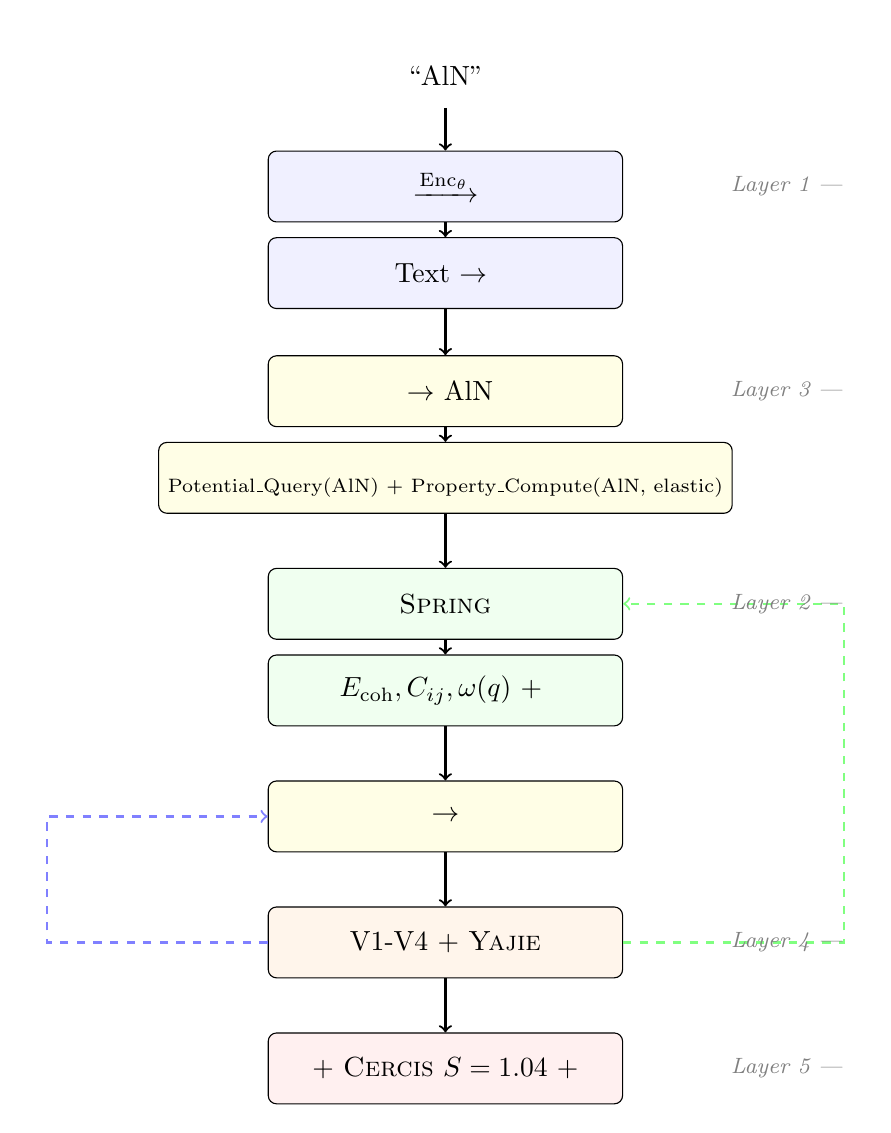
\begin{tikzpicture}[node distance=1.6cm, auto,
    block/.style={rectangle, draw, minimum width=4.5cm, minimum height=0.9cm, align=center, rounded corners=3pt},
    arrow/.style={->, thick}]

    % User
    \node[font=\bfseries] at (0, 2.2) {};
    \node[text width=4.5cm, align=center] at (0, 1.7) {“AlN”};

    % Layer 1
    \node[block, fill=blue!6] (l1a) at (0, 0.3) {\textbf{}$\xrightarrow{\Enc_\theta}$};
    \node[block, fill=blue!6] (l1b) at (0, -0.8) {Text $\to$ };

    % Layer 3 (reasoning - called first for text)
    \node[block, fill=yellow!10] (l3a) at (0, -2.3) {\textbf{} $\to$ AlN};
    \node[block, fill=yellow!10] (l3b) at (0, -3.4) {\\
        \scriptsize Potential\_Query(AlN) + Property\_Compute(AlN, elastic)};

    % Layer 2 (physics - triggered by reasoning)
    \node[block, fill=green!6] (l2a) at (0, -5.0) {\textbf{}\Spring{}};
    \node[block, fill=green!6] (l2b) at (0, -6.1) {$E_{\text{coh}}, C_{ij}, \omega(q)$ + };

    % Layer 3 again
    \node[block, fill=yellow!10] (l3c) at (0, -7.7) {\textbf{} $\to$ };

    % Layer 4
    \node[block, fill=orange!8] (l4a) at (0, -9.3) {\textbf{}V1-V4 + \Yajie{}};

    % Layer 5
    \node[block, fill=red!6] (l5) at (0, -10.9) {\textbf{} + \Cercis{} $S=1.04$ + };

    % Arrows
    \draw[arrow] (0, 1.3) -- (l1a);
    \draw[arrow] (l1a) -- (l1b);
    \draw[arrow] (l1b) -- (l3a);
    \draw[arrow] (l3a) -- (l3b);
    \draw[arrow] (l3b) -- (l2a);
    \draw[arrow] (l2a) -- (l2b);
    \draw[arrow] (l2b) -- (l3c);
    \draw[arrow] (l3c) -- (l4a);
    \draw[arrow] (l4a) -- (l5);

    % Feedback arrows
    \draw[arrow, blue!50, thick, dashed] (l4a.west) -- ++(-2.8,0) |- (l3c.west)
        node[pos=0.3, left, font=\footnotesize] {};
    \draw[arrow, green!50, thick, dashed] (l4a.east) -- ++(2.8,0) |- (l2a.east)
        node[pos=0.3, right, font=\footnotesize] {};

    % Layer labels
    \node[font=\footnotesize\itshape, right, text=gray] at (3.5, 0.3) {Layer 1 — };
    \node[font=\footnotesize\itshape, right, text=gray] at (3.5, -5.0) {Layer 2 — };
    \node[font=\footnotesize\itshape, right, text=gray] at (3.5, -2.3) {Layer 3 — };
    \node[font=\footnotesize\itshape, right, text=gray] at (3.5, -9.3) {Layer 4 — };
    \node[font=\footnotesize\itshape, right, text=gray] at (3.5, -10.9) {Layer 5 — };

\end{tikzpicture}
\caption{\Spring{}AlN}
\label{fig:pipeline_detail}
\end{figure}

\section{B}

\begin{table}[H]
\centering
\caption{}
\renewcommand{\arraystretch}{1.3}
\begin{tabular}{@{}p{2.5cm} p{4cm} p{7cm}@{}}
\toprule
\textbf{} & \textbf{} & \textbf{/} \\
\midrule
$\ModalitySet$ &  & $\{\text{DFT}, \text{MD}, \text{Text}, \text{Image}, \text{Audio}, \text{Video}, \text{Tabular}\}$ \\
$\Enc_\theta$ &  &  $\to \R^d$ \\
$\phi_m$ &  & $m$ \\
$V_{\text{consensus}}$ & \Spring{} & $M_t$ \\
$M_t$ / $\Mauto$ &  &  \\
$s_{\Yajie}$ & \Yajie{} & $[0,1]$ \\
$\Lyap_t$ & Lyapunov &  \\
$S_{\Cercis}$ & \Cercis{} & $Q_{\text{prec}} + \eta \cdot N_{\text{cov}}$ \\
$Q_{\text{prec}}$ &  & \Yajie{} \\
$N_{\text{cov}}$ &  &  \\
$\mathcal{T}_{\text{audit}}$ &  &  \\
$\Dhash$ &  & SHA-256 \\
$\Sigma_0(\D)$ &  &  \\
\bottomrule
\end{tabular}
\end{table}

\end{document}
